\section{Introduction}

Runtime verification (RV)  \cite{bartocci18,havelund-rv-data-2018} very generally refers to the use of rigorous (formal) 
techniques for {\em processing} execution traces emitted by a system being observed. The purpose is typically
%, again generally viewed, 
to evaluate the state of the observed system. Processing can take numerous
forms. We focus here on {\em specification-based} runtime verification, where an execution trace is checked against a property expressed in a formal logic, in our case variants of linear temporal logic.

Linear Temporal Logic (LTL) is a common specification formalism for reactive and concurrent systems. It is often used in e.g. model checking and runtime verification. Another formalism that is used for the same purpose is finite automata, often over infinite words. This includes B\"{u}chi, Rabin, Street, Muller and Parity automata~\cite{Thomas}, all having the same expressive power. In fact, model checking of an LTL specification
is usually performed by first translating the specification into a B\"{u}chi automaton. The automata formalisms are more expressive than LTL, with a classical example By Wolper~\cite{Wolper} showing that
it is not possible to express in LTL that every even state in
the sequence satisfies $p$. This has motivated extending LTL
in various ways.
We are mainly motivated by runtime verification of executions with data, for which a first-order temporal logic is
appropriate. There, too, we show that expressiveness can be extended.

We present first an extension of the propositional LTL that is based on using additional (auxiliary) propositions, not appearing in the execution, which summarize the past 
of the current execution. These propositions obtain their value in a state as a function of the prefix of the execution up and including that state through a past temporal formula. This can be seen as adding
summary states to the temporal specification, resulting in a specification that is in between logic and finite automata representation. This extension, which we believe is conceptually simpler
and more intuitive than other suggested extensions, is shown to be
equivalent to the other common specification formalism:
B\"{u}chi automata, regular expressions and quantified LTL.

We then proceed to first-order LTL. We relativise Wolper's example to the first
order case to motivate the need for
extending first-order LTL. Another example is based on the inexpressiveness of transitive closure of a relation in first order logic.
We present an extension where auxiliary relations, not appearing in the model, are
added. While this extension
is capable of expressing the above
properties, we show that for the first-order version, this has less 
expressive power than adding quantification over relations, in distinction from the corresponding propositional case.

These extensions to the logics are in particular natural for
runtime verification of past (safety) temporal properties, since
the values of propositional and first-order LTL are based
on calculating and updating a summary of the prefix of the execution. Runtime verification often concentrates on a past  version of temporal logic~\cite{HR} mainly because for these properties we can decide when the monitored property is violated immediately when this happen, while for future properties we may never know for sure. Consistent with that, 
we provide runtime verification algorithms for the past-time versions of the extended propositional and first-order
logics. We further present an extension of the 
\dejavu{} tool (https://github.com/havelund/dejavu) that
realizes the extended first-order past temporal logic verification. The \dejavu{} tool~\cite{HPU,HP} allows runtime verification on past time first order temporal logic over infinite domains (e.g., the integers, strings). It achieves efficiency by BDD representation of enumerations of data (rather than over the data values themselves) and using
a garbage collection algorithm. 
Finally, we provide some experimental results.

The contributions of this paper are both theoretical and practical. On the theory side, we present and study extensions for propositional and first order linear-temporal logics and show the relations between them and existing versions. 
On the practical side, we present algorithms for the extended logic, and 
show how to cast them specifically in an efficient BDD-based implementation. We present some experiments performed with our implementation and report on the results. 

The structure of this paper is as follows. In Section~2 we first define the syntax and semantics of propositional temporal logic. We then review some of its classical extensions and present our own extension. In Section~3 we present a runtime verification algorithm for the extended past LTL. In Section~4 we review first order linear temporal logic, present our extension and study the relationships between the presented versions of first-order LTL. IIn Section~5 we present a runtime verification algorithm for the past version of the extended first-order LTL. Section~6 describes the implementation and provides experimental results. Finally, Section~7 concludes the paper.

%\klaus{I think that the structure of the paper should be
%crystal clear so that the reader does not get lost. A lost reader leads to rejection. If a reader understand the structure, but perhaps not the details, the reader may still be happy.}

\vspace{1ex}
\noindent {\bf Related Work}
For propositional LTL, the logic ETL~\cite{WVS,Wolper} extends
the set of temporal operators 
by using automata (or, equivalently a right linear grammar). Each automaton defines a temporal operator,
where the input letters of the automaton correspond to future temporal subformulas. Each accepted run defines then the places
where the subformulas (corresponding to the occurrences of the input letters in the run) need to hold. Another expressive-equivalent extension, 
in~\cite{Wolper}, adds
state-dependent quantification over propositions to LTL.

Addition of relations to temporal databases is done
for aggregation~\cite{Libkin}, where relations are
calculated, based on the current state, and are used for further calculating
functions (sums, maxima) over the sequence of states. Aggregations were also used in the runtime verification tool 
{\sf MonPoly}~\cite{agrebasin}.
%
% --- other less directly related work: ---
%
Numerous other systems have been produced for monitoring
execution traces against formal specifications. 
These include e.g. \cite{Meredith2011,larva,Reger2015,halle-beepbeep-ieee-12,LOLA}. 

% ----------------

\iffalse
The contributions of the papers are both theoretical, and
practical. We study the extensions of propositional temporal logic (both full version and past/safety version) and suggest a restricted (and, to our opinion, an intuitive) extension that is equivalent to the power of quantified LTL or B\"{u}chi/finite automata. We then study 
The corresponding extension to first-order LTL, replacing propositions with relations, and allowing variables and constant values. We propose, for the first-order version, an extension similar to the one we propose for the propositional case. But then we show that for the first-order case, this extension has
less expressive power than adding quantification in the style of propositional temporal logic.

The extensions we suggest are in particular easy to implement, as an extension to existing propositional/first-order runtime verification. We extend our tool \dejavu, experiment with new examples that take advantage of the extension.
\fi
\vspace{1ex}
\noindent {\bf conventions}
\label{sec:prelim}
In this paper, we treat and present several versions of the logic LTL. To simplify
the presentation, we prefix LTL with letters as follows:

\begin{itemize}
\item{P} restricts to {\em past} temporal operators.
\item{F} allows first-order quantification over
variables and relations over variables and constants. This is referred to as {\em static} quantification.
\item{Q} adds quantification over predicates (for the propositional versions)
or over relations (for the first-order version). These objects can have different values at different states. This is referred to as {\em dynamic} quantification.
\item{E} allows extending the objects that occur in the input with
new auxiliary predicates (for the propositional versions) or relations (for the first-order cases).
\end{itemize}

\klaus{You above introduce some concepts before they really are explained. Q and E. I understand why you do this (to have it in one place), but it may be too difficult for the reader to grasp if not "initiated".
Especially the E.}

\klaus{We use ELTL (etc) to denote Extended LTL. 
But QLTL is also an extension of LTL. These logics 
are all extensions of LTL. Perhaps RLTL (for Rule-based 
LTL) would have been better ... or something. Not urgent, 
we can always change that if we want to.}

%\klaus{The explanation of Q and E could be improved.}


\newcommand\eventty{\mathbb{E}}
\newcommand\setof[1]{\mathcal{P}(#1)}


\section{Propositional LTL}

The classical definition of linear temporal logic~\cite{MP} has the following syntax:
\[ \varphi ::= \true \, | \,  p \, | \, ( \varphi \wedge \varphi ) \, |  \, \neg  \varphi \, |   \, \bigcirc \varphi \, |  
\, ( \varphi \until \varphi ) \,|  \, \ominus \varphi |
   \, ( \varphi \since \psi ) \,  \]
where $p$ is a proposition from a finite set of propositions $P$, and with $\bigcirc$, $\until$, $\ominus$, $\since$ standing for {\em next-time}, 
{\em until}, {\em previous-time} and {\em since}, respectively.


The models for LTL formulas 
are infinite sequence of states.
$\sigma =  s_{1}\, s_{2}\, s_3 \ldots$,
where $s_i \subseteq P$ for each $i\geq 0$. These are the propositions that {\em hold} in that state.
We denote by $\xi_{i}$ the suffix $s_{i} s_{i+1} s_{i+2}\ldots$ of $\sigma$. 
LTL's semantics is defined as follows:
\begin{itemize}
\item $( \sigma, {i}) \models \mathit{true}$.
\item $(\sigma, {i}) \models p$ iff $p \in s_{i}$.
\item $(\sigma, {i}) \models \neg\varphi$ iff  $(\sigma, {i}) \not\models \varphi$.
\item $(\sigma, {i}) \models ( \varphi \land \psi)$ iff $(\sigma, {i}) \models \varphi$ and $(\sigma, {i} ) \models \psi$.
\item $(\sigma, {i}) \models \bigcirc \varphi$ iff $(\sigma, {i+1}) \models \varphi$.
\item $(\sigma, {i}) \models ( \varphi\ \cal{U}\ \psi )$ iff for some 
$j\geq i$, $(\sigma, {j}) \models \psi$,
and for all $i \leq k < j$, $(\sigma, {k}) \models \varphi$.
\item $(\sigma , i) \models \ominus \varphi$ iff $| \sigma | > 1$ and $(\sigma, i-1) \models \varphi$.
\item $(\sigma , i) \models (\varphi \since \psi)$ iff there exists $1 \leq k \leq i$ such that
$(\sigma , i) \models \psi$  and for each
$j < k \leq i$, 
$(\sigma , k)  \models \psi$.
\end{itemize}
Then $\sigma \models \varphi$ when $( \sigma ,0 ) \models \varphi$.
We can use the following abbreviations:
$\false = \neg \true$, 
$(\varphi \vee \psi) = \neg ( \neg \varphi \wedge \neg \psi )$, 
$(\varphi \rightarrow \psi) = ( \neg \varphi \vee \psi)$,
$(\varphi \leftrightarrow \psi) = ((\neg \varphi \wedge \neg \psi) \vee (\varphi \wedge \psi ))$,
$\Diamond \varphi = (\true \until \varphi)$ and $\Box \varphi = \neg \Diamond \neg \varphi$,
${\bf P}\  \varphi = (\true \; \since \; \varphi)$, and 
${\bf H}\ \varphi = \neg {\bf P}\ \neg \varphi$.



%%infinite sequences (finite executions can be extended by repeating the last event indefinitely to form an infinite paths).
The expressive power of propositional LTL is often compared to regular expressions
over the alphabet $\Sigma = 2^P$ and to  {\em monadic} logics where the temporal propositions
correspond to unary predicates (over time). A full overview appears in~\cite{Thomas}. Accordingly, we have the following characterizations:
LTL is equivalent to monadic first-order logic\footnote{First-order logic with unary predicates over the naturals, and the relation $<$.},  star-free regular expressions\footnote{Regular expressions with the following operators: constant letters, concatenation and complementation, but no star (or $\omega$-star for infinite words).} and counter-free B\"{u}chi automata\footnote{A counter-free language is a regular language for which there is an integer n such that for all words x, y, z and integers $m \geq n$ we have that $xy^m z \in L$ if and only if $xy^n z \in L$.}. In fact, restricting the temporal operators to the {\em future}  operators $\until$ and $\bigcirc$
(and the ones derived from them $\Box$ and $\Diamond$)
leaves the same expressive power and is commonly used. 

%\klaus{Is that also the true for the first-order case? Doron: I have no idea. But at this point, I would not ask to ask Gabbay.}

An important subset of LTL, called here PLTL, allows only past temporal
operators: $\since$, $\ominus$ and the ones derived
from them $\mathbf{H}$ and $\mathbf{P}$. The logic is often
(and also here) interpreted over finite sequences, 
where $\sigma \models \varphi$ when $( \sigma , | \sigma | ) \models \varphi$.
Alternatively,
it is also a common practice to prefix the property with a single $\Box$ (always) operator, where each of the prefixes has to satisfy $\varphi$. This later
form expresses {\em safety} properties~\cite{AS} over infinite sequences. 



When PLTL is interpreted over finite sequences, its
expressive power is the same as star-free regular expressions, first-order monadic logic over finite sequences and counting-free automata.


\section*{Extending Propositional LTL}
\label{sec:extending-prop-ltl}

\subsubsection{Extending with Dynamic Quantification}

Wolper~\cite{Wolper} showed that the expressive power of LTL is lacking with respect
to some important properties. As a canonical example, he demonstrated that it is impossible to
express that all the states with even indexes of a sequence
satisfy $p$ (this is
different than saying that $p$ alternates between $\true$ and $\false$ on consecutive states). In order to extend the expressiveness of LTL, Wolper suggested to use linear grammars, or, alternatively, the ability to quantify over
propositions. 


Adding quantification over propositions allows writing a formula of the form
$\Exists q \, \varphi$, where $q$ is a proposition that can appear in $\varphi$.
Let the propositions $P$ be partitioned into two disjoint sets: 
{\em auxiliary propositions} $A = \{ a_1 , \; \ldots\; , a_n \}$
and {\em basic propositions} $B$. 
%A model for such a formula 
%has truth assignments only over the propositions in $B$, but the propositions $A$ can appear (only) within the scope of a quantifier.
We also allow $\Forall q\, \varphi =
\neg \Exists q\, \neg \varphi$.
To define the semantics, let $X$ be a subset of 
the propositional variables appearing in the states of the sequence $\sigma = s_1 s_2 \ldots$ and 
denote $\sigma |_X = s_1 \setminus X \, s_2 \setminus X \ldots$. (Note that $\sigma |_X$ denotes projecting {\em out} the variables in $X$.)



\begin{itemize}
\item $( \sigma, i ) \models \boldsymbol{\Exists} q \, \varphi$ iff there exists
$\sigma'$ such that $\sigma' |_{\{ q \} } = \sigma$ and 
$( \sigma', i) \models \varphi$.
\end{itemize}
Since all the auxiliary variables appear in the scope of
quantifiers, it holds that $\sigma \models \varphi$
(in $\varphi$, auxiliary variables appear only within
the scope of quantifiers)
iff $\sigma |_A \models \varphi$.

\klaus{Are the last two lines above needed?}

This kind of quantification is considered to be ``dynamic'', since the quantified variables can have different truth values depending on the states, or, "second order", the quantification establishes the {\em set} of states in which a propositional variable has the value $\true$.
Extending LTL with such quantification, the logic QLTL has the same expressive power as regular expressions, full B\"{u}chi
automata, or monadic second order logic with unary predicates over the naturals, see again~\cite{Thomas}.
In fact, it is sufficient to restrict the quantification to existential quantifiers that prefix the formula to obtain the full expressiveness of QLTL~\cite{Thomas}. 

\noindent
Wolper's property can be expressed in QLTL as follows:
\begin{equation} \label{form0} \Exists q \,
( (  \neg q \wedge \Box (q \leftrightarrow \bigcirc \neg q )  )  \wedge \Box (q \rightarrow p ) )\end{equation}
Wolper's example property cannot be expressed in PLTL either.

If we allow
quantification over propositions, we obtain the logic PQLTL
(QLTL restricted to the past modalities), with the following formula:
\begin{equation} \label{form1} \Exists q \,
{\bf H} (( q \leftrightarrow \ominus \neg q )   \wedge (q \rightarrow p ) )\end{equation}
%In fact, it can be shown that a single existential quantifier is sufficient. 
PQLTL has the same expressive
power as regular expressions and finite automata.
Note that since finite automata over finite sequences can be determinized, it is always sufficient to translate a
PQLTL property into a deterministic
automaton.


\subsubsection{Extending with Rules}

We present now an extension of LTL, which we call ELTL. It has the same
expressive power as  QLTL.
It has a form that puts it, conceptually, in between temporal
logic and automata: on the one hand, it is possible to simply write
a pure LTL formula, and on the other hand, one can write a specification that resembles a finite automaton. As will be showed later, this extension is
is very natural for runtime verification.

We partition again, as in QLTL, the propositions $P$ into
{\em auxiliary propositions} $A = \{ a_1 , \; \ldots\; , a_n \}$
and {\em basic propositions} $B$. A model for an ELTL formula has truth assignments only over the propositions in $B$.
An ELTL property $\eta$ has the following form: 
\begin{equation} \label{ELTL}
\psi \mathit{\ where\ } a_j  := \varphi_j \, : \, 
 {j \in \{1, \ldots , n\}} \end{equation}
where each $a_i$ is a distinct auxiliary proposition from $A$,
$\psi$ is an LTL property and each $\varphi_i$ 
is a PLTL property where propositions from $B$ can
only occur within the scope of a $\ominus$ operator.
The semantics can be defined as follows. We refer to $\psi$
as the {\em statement} of $\eta$ and to 
$a_j  := \varphi_j \, : \, 
 {j \in \{1, \ldots , n\}}$ as the rules. In text, rules
 will be separated from each other by a comma (",").

\begin{tabbing}
\ \ \ $\sigma \models \eta$ \=  if there exists $\sigma'$, where
$\sigma' |_A = \sigma$ such that \\
 \> $\sigma' \models ( \psi  \wedge   \Box \bigwedge_{1 \leq j \leq n} ( a_j \leftrightarrow \varphi_j)) $
\end{tabbing}

\noindent
Wolper's example can be written in ELTL
as follows:
\begin{equation} 
\label{form3}
\Box ( q \rightarrow p ) \, \mathrm{where} \, 
 ( q := \ominus \neg q)
\end{equation}
where $A = \{ q\}$ and $B = \{ p \}$.
The auxiliary variable $q$ is used to augment the input sequence such that each {\em odd} state will satisfy $\neg q$
and each {\em even} state will satisfy $p$.  As $\ominus \varphi \models \false$ in the initial state, regardless of $\varphi$, then
$q$ is $\false$ in the initial state, and then it subsequently alternates.


ELTL extends the set of propositional variables with new variables whose values at a state are
based on the prefix of the model. We say that
the extension of the states are {\em well founded},
as the added propositions are dependent and effectively summarize the past execution prefix up to and
including the current state.
This differs from 
the use of auxiliary variables in QLTL, where the auxiliary variables do not have to extend the execution
states in a fixed way throughout the interpretation of 
the property over a model. The constraint that auxiliary variables appearing in the formulas $\varphi_i$ 
must occur within the scope of a $\ominus$ operator
is required to guarantee that the values
of the auxiliary variables are not conflicting, as in
$a_1 = \neg a_2$ and $a_2 = a_1$, which makes a formula
that uses $a_1$ and $a_2$ uniformly $\false$.

\begin{lemma} \label{fourone}
Let $\varphi$ be an ELTL formula as in~(\ref{ELTL}),
over the auxiliary propositions $A$ and basic propositions $B$, 
and let $\sigma$ be a model with states over the $B$, such that
$\sigma \models \psi$.
Then there is a unique
model $\sigma'$ such that $\sigma' |_A = \sigma$.

\end{lemma}

\klaus{(1) is this lemma saying the right thing? (2) is the proof really a proof of that lemma, (3) 
should $\varphi$ be $\psi$, (4) now $\psi$ is not the whole spec (it is missing the rules). What do we call the whole thing? It is not a formula like the 
$\varphi$s and the $\psi$s. Do we need a special greek symbol for it?}

\noindent {\bf Sketch of proof.} By induction on the state index. Each auxiliary variable
is defined, via a PLTL formula by the current state of the model over the values of the propositions $B$, and by the values of $A \cup B$ in previous states. A PLTL
property depends on a state only on the prefix
of the model that precedes and includes that state.
Restricting the auxiliary variables to appear only within the scope of a previous-time operator guarantees that
their values at the current state cannot be conflicting. \qed


\begin{theorem}
\label{theo1}
The expressive power of 
ELTL is the same as QLTL.
\end{theorem}
\noindent {\bf Proof.}
Each ELTL formula $\eta$, as defined above,
is expressible in QLTL using the following formula:

\[   \Exists a_1 \ldots \Exists a_n  ( \psi  \wedge   \Box \bigwedge_{1 \leq j \leq n} ( a_j \leftrightarrow \varphi_j))
\]

\klaus{How do we know that the ``other direction'' below is possible?}

For the other direction, one can translate any QLTL property into an $\omega$ automaton\footnote{The past operators of a QLTL property do not change this fact, since the translation can be done first to second order monadic logic, which can be translated into an $\omega$-automaton.}.
We assume that the property is given as a deterministic Muller automaton $M = (S, i , \Sigma, \Delta, {\cal F})$ (a B\"{u}chi automaton may not always be deterministic), where $S$ is the set of states, $i \in S$ is the initial state, $\Sigma$ is the set of inputs, each represented as a Boolean combination of the variables $B$, $\Delta : S \times \Sigma \mapsto S$ is the transition function, and ${\cal F} = \{ F_1 , \ldots , F_k \}$ is the accepting set, 
where an accepted input needs to pass infinitely often in exactly
one of the specified sets. To formulate an ELTL formula,
he auxiliary variables represent the states $S$ of $M$, i.e., $a_s$ represents the state $s \in S$.

\klaus{The following formulation above is not not clear: ``where an accepted input needs to pass infinitely often in exactly
one of the specified sets''.}

\noindent
Then we translate $M$ into an ELTL formula
of the form: 

\begin{tabbing}
\ \ \ \ \ $\bigvee_{F \in {\cal F}} (\bigwedge_{s \in F} \Box\Diamond a_s \wedge \bigwedge_{s \not\in F} \Diamond \Box \neg a_s)$
where \\
\ \ \ \ \ \ \ \ \ \ $a_s := \vee _{\Delta ( s'
, \alpha ) = s } 
\alpha \wedge \ominus a_{s'} )
\wedge (s=i \rightarrow \neg \ominus \true)
\, :\,  s \in S
$
\end{tabbing}

\klaus{Above: should $s=i \rightarrow \neg \ominus \true$ instead be (note: two changes):
$\neg \ominus \true \rightarrow a_s=i$
}

\klaus{Above: can't judge whether the $\bigwedge_{s \not\in F} \Diamond \Box \neg a_s)$ is correct.}

\noindent
With $(s=i)$ is $\true$ when $s$ is $i$, and $\false$ otherwise.
Basically, the assignments to the auxiliary variables are used to simulate the change of states\footnote{It is possible to use only $\lceil \log ( | S | ) \rceil$
variables, at the expense of longer and more complicated formulas.}, and the main formula expresses the Muller acceptance condition. \qed

The use of the auxiliary variables $a_1 \ldots a_n$ in the
rules of an ELTL specification 
$\eta$ can be viewed as representing a
state machine, in particular when the only modality that is used in the rules part is $\ominus$.
In that case, we can consider an ELTL specification $\eta$ as consisting with two synchronous parts: an LTL property 
(the statement) $\psi$
and a finite automaton, whose states correspond to combinations
of truth values of the auxiliary variables, and can be referred to
within $\psi$. As a corollary of Theorem~\ref{theo1}, 
this restricted representation is also equivalent to QLTL.
This representation can be useful, for RV, as explored further in this paper, because of the possibility to
incrementally calculate the values of the auxiliary variables. 
Similarly, it can be
used for extending the expressiveness of LTL model checking.

\klaus{First sentence below sounds wrong: (1) PLTL already does not have future time operators, and (2) why mention infinite sequences?}

We can extend PLTL into EPLTL by disallowing the future temporal operators (except a prefixing $\Box$, when interpreted over infinite sequences). We obtain
a formalism that is equivalent to finite automata. In this case, 
we replace the first part of the construction in the proof of Theorem~\ref{theo1}
with the simpler formula $\vee_{s \in A} a_s$, where $A$ are the accepting states of the finite automaton.

\klaus{Last sentence above: perhaps say with words that we are always in an acceptance state - if that's what the point is.}

For representing safety properties that can be expressed in QPLTL, we can use a restricted version as shown in the following simple Lemma.
\begin{lemma}
\label{simplecase}
Any safety QPLTL property can be expressed using the following restricted
ELTL form:
\[  \Box p {\ where\ } a_j  = \varphi_j \, : \, 
 {j \in \{1, \ldots , n\}}  \] 
 with $p$ being one of the auxiliary variables $a_j$.
\end{lemma}
\noindent {\bf Proof.} The proof of the Lemma follows from the
axiomatization of QLTL in~\cite{MP}, e.g.,
$\varphi\ \since\ \psi \leftrightarrow \psi \vee ( \varphi \wedge (\varphi\ \since\ \psi))$. \qed

\klaus{In the axiom above, isn't there missing a $\ominus$ before
the second $(\varphi\ \since\ \psi)$?}

\klaus{Above: is the following really correct?: 
``with $p$ being one of the auxiliary variables $a_j$''.}

While this Lemma makes the use of the temporal operators
besides $\ominus$ redundant, we believe that it is still
more convenient to use a combination of
temporal operators when possible, and
auxiliary variables definitions.
The relative expressive power between the propositional temporal logics discussed here
appear in Figure~\ref{prop}.






\begin{figure}
\begin{center}
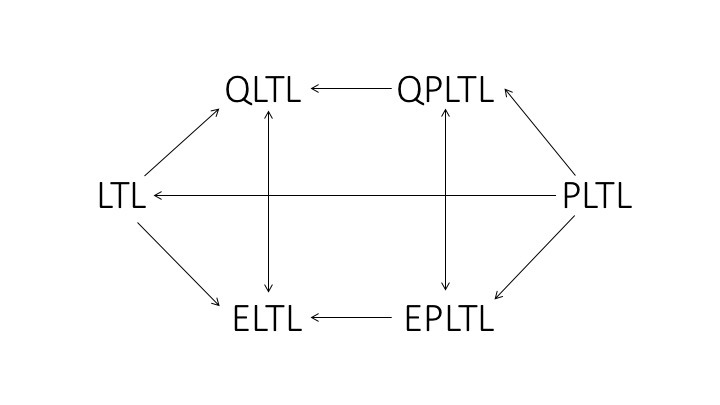
\includegraphics[height=1.1in,width=2.7in]{PROP.jpg}
\caption{\label{prop} An arrow from A to B means that logic  B is more expressive than A. A double headed arrow shows same expressiveness}
\end{center}
\end{figure}




\section{RV for Propositional Past-Time LTL and its Extension}
\label{LTLruntime}

Runtime verification of temporal specifications often
concentrates on the past portion of the logic.  Past-time  specifications have the important property that one can distinguish when they are violated. For an extended discussion of this issue of {\em monitorability}, see e.g.,~\cite{Ugly,FFM}.

The algorithm for PLTL, first presented in \cite{HR}, 
is based on the observation that the semantics of the 
past time formulas $\ominus \varphi$ and $(\varphi\, \since \,\psi)$ in the current step $i$ is defined in terms of the semantics
in the previous step $i - 1$ of a subformula.
To demonstrate this, we repeat here the definition of the previous-time
operator $\ominus$, and rewrite the definition
of $\since$ in an equivalent form that is
more directly amenable for runtime verification.

\begin{itemize}
\item $( \sigma , i) \models \ominus \varphi$ iff $i > 1$ and $(\sigma, i-1) \models \varphi$.
\item $(\sigma , i) \models (\varphi \, \since \, \psi)$ iff $(\sigma , i) \models \psi$ or the following hold: $i>1$,
$( \sigma , i)  \models \varphi$ and 
$(\sigma , i-1 ) \models ( \varphi \, \since \, \psi )$.
\end{itemize}

\noindent
Runtime verification exploits the fact that
the semantic definition is recursive in both the structure of the property, where subformulas
are evaluated based on smaller subformulas, and the
evaluation of subformulas in the previous state.
The algorithm, shown below, operates on two vectors (arrays) of values indexed by subformulas:  $\old$ that summarizes the truth values of the
subformulas just {\em before} the new state, and $\current$ for the {\em current} state.

\begin{enumerate}
\item Initially, for each subformula $\varphi$,
%$B ( \varphi , \current ) = \bfalse $.
$\current ( \varphi ) := \false$.
\item Observe a new event (as a set of ground predicates) $s$ as input. 
\item Let $\old := \current$.
\item Make the following updates for each subformula. If $\varphi$ is
      a subformula of $\psi$ then $\current ( \varphi )$ is updated before 
      $\current ( \psi )$.

\begin{itemize}
  \item $\current ( \true ) := \true$.
  \item $\current (  \varphi \wedge \psi  ) := 
  \current ( \varphi )\  and\ \current ( \psi )$.
  \item $\current ( \neg \varphi  ) := not\ \current ( \varphi )$.
  \item $\current (  \varphi \since \psi  ) :=  
  \current ( \psi  )\ or\ ( \current ( \varphi ) \ and\ 
      \old ( ( \varphi \since  \psi )))$.
%DAP: I removed the \; around \since, since it penetrated the 2nd column!
  \item $\current ( \ominus \; \varphi ) := \old ( \varphi )$.
  
\end{itemize}
\item Goto step~2.
\end{enumerate}

\noindent
Runtime verification of QPLTL can be done by translating a
formula into a deterministic finite automaton. Then the sequence of states to be checked forms the input for this automaton. 
However, QPLTL can be extremely compact, in particular when using alternating existential and universal 
quantifiers, which can result in a huge (non-elementary) explosion of
the automaton representing the same
specification~\cite{Thomas}.

The well foundedness of the formulas defining the new auxiliary variables in EPLTL makes the extension of the above
runtime algorithm simple.
In order to extend the algorithm to perform runtime verification of an EPLTL formula $\psi$, as defined in~(\ref{ELTL}),  we need to  add to the above
algorithm memory for $\current ( a_j )$ and $\old ( a_j )$,
and perform the following between steps 3 and 4 for each $a_j$: \\

\ \ \ \ \ $\current ( a_j ) := \current ( \varphi_j )$ \\

\subsubsection{Evaluation Order} 

The order of calculating $\current$ is subtle here, because
auxiliary variables can appear recursively on the right-hand 
side of their definition. For PLTL, one can start calculating the subformulas
bottom up or top down. But for EPLTL, this would not work. To see this, consider, for example, the formula~(\ref{form3}). It contains
the definition $q := \ominus \neg q$. Now, we cannot calculate this
bottom up, since the left-hand $q$ is not calculated yet, and we need its value to compute the right-hand side $q$ leaf node.
If we calculate it top down, we will encounter the same problem.
However, notice that the top down calculation does not need the
value of $q$ to calculate $\ominus \neg q$; this value should already be available as $\old ( \neg q )$.

\klaus{I don't see that we need to talk about the top-down evaluation.}

Under {\em mixed evaluation order}, one calculates $\current$ in the following order. The calculation within each of the four categories can be performed top down or bottom up.

\begin{enumerate}
\item Calculate 
$\current ( \delta )$ for each subformula $\delta$
that appears in $\varphi_j$ of rule
$a_j := \varphi_j$ but not within the scope of
a $\ominus$ operator. (This is not
a problem since for $\delta = \ominus \gamma$,
$\current ( \delta )$ is set to $\old ( \gamma )$.)
\item Set 
$\current ( a_j )$ to $\current ( \varphi_j )$ for each $j$.
\item Calculate $\current ( \delta )$ for each subformula $\delta$
that appears in $\varphi_j$ of a rule
$a_j = \varphi_j$ {\em  within} the scope of
a $\ominus$ operator.
\item Calculate $\current ( \delta )$ for each subformula $\delta$
that appears in the statement $\psi$ - using $\current ( a_j )$.
\end{enumerate}



\section{First-Order LTL}

%section*{Syntax and Semantics}
\label{sec:syntax-semantics}

Assume a finite set of infinite domains\footnote{Finite domains are handled with some minor changes, see~\cite{HPU}.}
$D_1, D_2, \ldots$,
e.g., integers or strings. 
Let $V$ be a finite set of {\em variables}, 
with typical instances $x$, $y$, $z$.
%We denote by $x: D$ the fact that the variable $x$ has the domain $D$.
An {\em assignment} over a set of variables $V$
maps each variable $x \in V$ to a value from
its associated domain $\domain ( x )$, where multiple variables (or all of them)
can be related to the same domain. For example
$[ x \rightarrow 5 , y \rightarrow \text{``abc''} ]$ assigns
the values $5$ to $x$ and the value ``abc'' to $y$.
Let $T$ be a set of {\em relations} 
with typical instances $R$.
Each relation is associated with some position-dependent domains.

\klaus{Above: let T be ... Is T used later? The relations are used in the next paragraph, why not introduce them there? Also, relations are not defined really.}

\klaus{I don't quite understand the motivation below for this way of modeling events: relations with a time stamp, and the whole story of the time stamp not being mentioned etc. Why not just the usual models: traces? Too late to change now for CAV though.}

We define models for FLTL based on {\em temporal} relations~\cite{Chomicki}. That is,
their last parameter
is a natural number. For a relation $R$, $R [ i ]$ is the relation obtained from $R$ by
restricting it to the value $i$ in the last parameter. For simplicity, we will describe henceforth
the logic with relations $R$ that have exactly two parameters, 
hence $R [ i ]$ will have just one parameter whose domain will be denoted as $d ( R )$; this domain is fixed over all the values of the second parameter $i$. The definition of the logic over other numbers of parameters is quite straightforward, and our implementation of runtime verification fully supports it.

\klaus{Above, what about instead of writing: ``this domain is fixed over all the values of the second parameter $i$'' to write:
``this domain is independent of the values of the second parameter $i$'' - if that is what you mean to say.}

\klaus{Above: we need to say explicitly what $i$ intuitively is meant to represent: positions, time, ....}

\subsubsection{Syntax} 

The formulas of the core FLTL logic are 
defined by the following grammar,
where $p$ denotes a relation $R$,
$a$ is a constant representing a value in $d ( R )$ and $x$ is a variable with $\domain ( x ) = d ( p )$.
\begin{center}
$\varphi ::= \true  \; | \;
    p ( a ) \; | \;
    p ( x ) \; | \;
    ( \varphi \wedge \varphi ) \;  |   \;
   \neg \varphi \; | \;
   \bigcirc \varphi \; | \; 
   ( \varphi \; \until \; \varphi ) \; | $ %\\
   $ \ominus \; \varphi \; | \;
    ( \varphi  \; \since  \; \varphi ) \; | \;
    \exists x \; \varphi$
\end{center}

%We interpret a predicate $p(a)$ as a subformula that
%represents the occurrence of some
%For example, if we open
%a file named $\text{``xyz''}$, we may have $\mathit{open}
%(\text{``xyz''})$, where the
%domain of the predicate ${\mathit{open}}$ is over strings representing
%file names.

\noindent 

Additional operators are defined as in the propositional logic. In addition we define
$\forall x \; \varphi = \neg \exists x \neg \varphi$.
Restricting the modal operators to the past ones
($\since$, $\ominus$ and the ones obtained from them) 
forms the logic PFLTL.
The quantification over values of variables here is `static' in the sense that values quantified over are independent of the state in the execution. We
denote static quantification with $\exists$ and $\forall$, while
dynamic quantification is expressed with $\Exists$ and $\Forall$
(see e.g. Section \ref{sec:extending-prop-ltl}).

\subsubsection{Semantics} 

A model is a set of
 relations ${\cal R} = \{ R_1 \, \ldots , R_m \}$, where each of these relations has a last parameter $i$ that is a natural number. 
% 
It is standard, and more intuitive (in particular for runtime verification) to cast models of temporal logic in terms of sequences states rather than temporal relations. To do that,
 we denote by $R_k [ i ]$ the restriction of
 the relation $R_k$ to the value $i$ of the last parameter. A model ${\cal R}$ is then a sequence ${\cal R} [ 1 ]\, {\cal R} [ 2 ] \ldots$, where
 each {\em state} ${\cal R} [i] = \{ R_1 [i], \ldots , R_m [ i ] \}$  (a set of relations).
 The denotation $p_k$ will correspond to the relation $R_k$.

\klaus{Above, did you not already say the following before:
``we denote by $R_k [ i ]$ the restriction of
 the relation $R_k$ to the value $i$ of the last parameter.''.}

\iffalse
At a given state the formula
$p(\text{``a''})$ means that $p (\text{``a''} )$ holds
in the current state,
that is, $p (\text{``a''} )$ is among 
the ground predicates of the state.
Consider now the formula $p ( x )$, for a variable $x \in V$.
We interpret it such that $x$ is assigned any value ``$a$'' where
$p ( \text{``a''} )$ appears in the current state. 
%DP: Added parentheses on the outside level.
Thus, for interpreting $(p ( x ) \wedge q ( y ))$ in a state that
has the predicates
$p ( \text{``a''} )$ and $q ( 3 )$,
we have the assignment $[ x \mapsto \text{``a''} , y \mapsto 3 ]$.
%The past time temporal operators have the following intuitive meaning.
The formula $(\varphi_1\; \since\; \varphi_2)$ 
(reads $\varphi_1$ {\em since} $\varphi_2$)
means that $\varphi_2$ occurred in the past (including now)
and since then (beyond that state) $\varphi_1$ has been true. This is the 
past dual of the commonly used %DP: changed "common" to "commonly used".
future time  {\em until} modality~\cite{MP}. 
The property $\ominus \; \varphi$ means that $\varphi$ is true 
in the previous state.
This is the past dual of the %DP: removed "common".
future time {\em next} modality.
We can also define the following additional temporal operators:
$P \; \varphi = (\true \, \since \, \varphi)$ (``previously''),
and $H \varphi = \neg P \neg \varphi$ (``always in the past'' or ``historically'').
The operator $[\varphi_1,\varphi_2)$, borrowed from \cite{MaC}, 
has the same meaning as $(\neg \varphi_2\; \since\; \varphi_1)$, but reads more naturally as
a semi-open interval. 



%Consider now the formula $P \neg p ( v )$, meaning that
%sometimes in the past $\neg p ( v )$. The semantics of $P$
%will be the union on the sets of values in the previous sets,
%thus, we need to take the union of $\neg p ( v )$ interpreted
%over all past states (including the current one).
%
%Suppose that we have the predicate $p ( i )$ at state $s_i$.
%There are several ways to interpret that.
%\begin{enumerate}
%\item We complement with respect to
%all the values in $domain ( p )$.
%Thus, the complementation will be $N \setminus \{ i \}$ at state $i$,
%where $N$ is the domain natural numbers, and the 
%$N \setminus \{ i \}$ from $1$ to $n$ is $N$.
%
%\item We complement with respect to
%the values in $domain ( p )$ that appeared so far in the sequence.
%Thus, at state $s_i$ we already saw $\{1 , \ldots , i \}$
%and as we see $p ( i )$ in the current state, the complementation 
%at state $s_i$ is $\{ 1, \ldots , i-1 \}$. The union 
%up to the $n$th state will give $\{1, \ldots , n-1 \}$.
%
%\item When new values appear later in the sequence, we 
%update the complementation related to previous states to include
%newly appearing values.
%Then we have to take the union of $n$ sets
%that do not include one distinct element each. This
%gives us at the $n$th state $\{ 1 , \ldots , n \}$.
%\end{enumerate}

%In our implementation we will take the first interpretation.
%However, we will assume that we have a reasonable
%limit on the number of different values that can appear in
%each domain. As it will cost us very little to assume quite
%a large size of values (the size of memory and amount of
%time of the implementation will be propositional to the
%{\em actual} number of values seen and not to this limit), we deem
%this assumption quite reasonable. %We will explain how to 
%remove this constraint (however, this requires quite a
%complicated implementation). It is also quite easy to see
%how to change the semantics to conform with case $1$ and
%how to implement it.


Let $\gamma$ be an assignment to the variables that appear
free in a formula $\varphi$.
Then $( \gamma ,  \sigma, i ) \models \varphi$
if $\varphi$ holds for the prefix $s_1 s_2 \ldots s_i$ of 
the trace $\sigma$
with the assignment $\gamma$. This is a standard definition,
agreeing, e.g., with~\cite{Basin}. Note that by using past %DP: appearing in, instead of appearing with.
operators, the semantics is not affected by
states $s_j$ for $j>i$.
%
\fi

Let $\vars ( \varphi )$ be the set of free (i.e., unquantified) variables of a
subformula $\varphi$. 
%The interpretation of a subformula
%$\varphi$ over some finite sequence is as a set of assignments
%to the variables $\vars ( \varphi)$.
We denote by $\gamma |_{\vars ( \varphi )}$ the restriction (projection) of
an assignment $\gamma$ to the free variables appearing in $\varphi$.
%We are careful in combining the sets of assignments
%between different
%subformulas, e.g., through union and intersection (corresponding
%to disjunction and conjunction, respectively) and the quantification.
%This is done using the projection and extension functions over
%assignments defined above.
%
Let $\epsilon$ be the empty assignment. 
%
In any of the following cases, $( \gamma,  {\cal R} , i ) \models \varphi$
is defined when $\gamma$ is an
assignment over $\vars ( \varphi )$, and $i\ge 1$.

\begin{itemize}

\item $( \epsilon , {\cal R} , i ) \models \true$.

\item $( \epsilon ,  {\cal R} , i )
 \models p_k ( a ) $ if $R_k ( a, i )$, where $a$ denotes a constant from  $d(p)$.

\item $( [ x \mapsto a ] , {\cal R} , i ) \models p_k ( x )$ if $R_k ( a , i )$.

\item $( \gamma,  {\cal R} , i ) \models ( \varphi \wedge \psi ) $~if~$(
\gamma |_{\vars  ( \varphi )} , {\cal R} , i ) \models \varphi$~and  \\
$( \gamma |_{\vars ( \psi ) } , {\cal R} , i ) \models \psi$. 

\item $( \gamma , {\cal R} , i ) \models \neg \varphi$ if not $( \gamma , {\cal R} , i ) 
\models \varphi$.

\item $( \gamma , {\cal R} , i) \models \bigcirc \varphi$ if 
$(\gamma , {\cal R} , i + 1) \models
\varphi$.

\item $( \gamma , {\cal R} , i ) \models ( \varphi \; \until \; \psi )$ if
for some $j > i$, $( \gamma |_{\vars ( \psi )} , {\cal R} , j) 
\models \psi $ and for all $i \leq k < j $,
$( \gamma |_{\vars ( \varphi )} , {\cal R} , k) \models \varphi$.


\item $( \gamma , {\cal R} , i) \models \ominus \varphi$ if $i>1$ and
$(\gamma , {\cal R} , i-1) \models
\varphi$.

\item $( \gamma , {\cal R} , i ) \models ( \varphi \; \since \; \psi )$ if
for some $1 \le j \leq i$, $( \gamma |_{\vars ( \psi )} , {\cal R} , j) 
\models \psi $ and for all $j < k \leq i$,
$( \gamma |_{\vars ( \varphi )} , {\cal R} , k) \models \varphi$.





\item $( \gamma , {\cal R} , i) \models \exists x \; \varphi$ if
there exists $a \in \domain ( x )$ such that\footnote{$\gamma \, [ x \mapsto a ]$
is the overriding of $\gamma$ with the binding $[ x \mapsto a ]$.}
$( \gamma \, [ x \mapsto a ], \sigma , i) \models \varphi$.

\end{itemize}

\iffalse
The definition of the {\em since} operator $S$ can be simplified in a standard
way such that it refers only to the positions $i$ and $i-1$ in
the sequence $\sigma$. This is based on the
fact that according to the semantics of {\em since},
$(\varphi \, \since \, \psi) = ( \psi \vee (\varphi \wedge \ominus 
(\varphi \, \since \, \psi )))$.
This will serve in the
implementation to work with only two versions of
the sets of assignments, for the current and previous state:

\begin{itemize}
\item $( \gamma , {\cal R} , i ) \models ( \varphi \, \since \, \psi )$ if
$( \gamma |_{\vars ( \psi )} , {\cal R} , i ) \models \psi$ or $i>1$,
$( \gamma |_{\vars ( \varphi )} , {\cal R} , i ) \models \varphi$, and \\
$( \gamma , {\cal R} , i-1 ) \models ( \varphi \, \since \, \psi )$.
\end{itemize}
\fi

%We can also define the following useful operators:
%$P \varphi = (\true \, \since \, \varphi)$ (for ``previously''),
%$( \varphi \, R \, \psi ) = \neg ( \neg \varphi \, \since \, \neg \psi )$ 
%(the dual of the Since operator), and
%$H \varphi = ( \false \, R \, \varphi )$ (for ``always in the past'').




%We define $\mathbf{F}$ and $\mathbf{T}$ as special constants
%in order to interpret formulas without free variables.
%They are the complement of each other.
%When combined with set operators (complementation, union, intersection),
%$\mathbf{F}$ behaves as the empty set, hence is idempotent to
%union. Accordingly, $\mathbf{T}$ is idempotent to intersection.

\iffalse
We denote by $A_{\vars ( \varphi )}$ the set of all possible assignments
of values to the variables that appear free
in $\varphi$. Thus,
$I [ \varphi, \sigma , i] \subseteq A_{\vars ( \varphi )}$.
To simplify definitions, we add
a dummy position $0$ for sequence $\sigma$ (which starts with $s_1$), 
where every formula is interpreted as an empty set.
Observe that the value $\emptyset$ and $\{ \epsilon \}$, behave
as the Boolean constants $0$ and $1$, respectively.
The set semantics is defined as follows, where $i \ge 1$.

\begin{itemize}
\item $I [ \varphi , \sigma , 0 ] = \emptyset$.
\item $I [ \true , \sigma , i ] = \{ \epsilon \}$.
\item $I [ p ( a ) , \sigma , i ] =$ if $p ( a ) \in \sigma [ i ]$ then
$\{ \epsilon \}$ else $\emptyset$.
\item $I [ p ( v ) , \sigma , i ] = \{ [ v \mapsto a ] \; | \; p ( a ) \in
\sigma [ i ] \}$.
%\item $I [ \true , \sigma , i ] = D^n$.
%\item $I [ ( \varphi \vee \psi ) , \sigma , i ] = 
%I [ \varphi , \sigma , i ] \cup I [ \psi , \sigma , i ]$.
\item $I [ ( \varphi \wedge \psi ) , \sigma , i ] = 
I [ \varphi , \sigma , i ] \;  \bigcap \; I [ \psi , \sigma , i ]$.
\item $I [ \neg \varphi , \sigma , i ] = 
A_{\vars ( \varphi )} \; \setminus \; I [ \varphi , \sigma , i ]$.
\item $I [ ( \varphi \; \since \; \psi ) , \sigma , i ] = 
I [ \psi , \sigma , i ] \; \bigcup \;
( I [ \varphi , \sigma , i ] \; \bigcap \; 
I [ (\varphi \since \psi ) , \sigma , i - 1 ] )$.
\item $I [ \ominus \varphi , \sigma , i ] = I [ \varphi , \sigma , i-1 ]$.
\item $I [ \exists x \; \varphi , \sigma , i ] = 
\proj ( I [ \varphi , \sigma , i ] , \{ x \} )$.
\end{itemize}

\noindent
As before, the interpretation for the rest of the operators can
be obtained from the above using the connections between the operators,
e.g., $I [ P \, \varphi  , \sigma , i ] = 
I [ ( \true \, \since \, \varphi ) , \sigma , i ]$.
The correspondence between this set based semantics 
and the previous semantics, namely that
$\gamma \in I [ \varphi , \sigma, i ]$ iff
$( \gamma , \sigma , i ) \models \varphi$
can be proved by a simple structural induction on
the size of the formulas.
 \fi

Then for an FLTL (PFLTL) formula with no free variables, ${\cal R} \models \varphi$ iff $( \epsilon , {\cal R} , 1 ) \models \varphi$.
We will henceforth sometimes abuse notation, as is very often done in logic, and use the same
symbols both for the relations (semantics) and their representation in
the logic (syntax).

\section*{Extending First-Order LTL}

%%this is specification formalism that is very expressive and yet monitorable under run time verification~\cite{HPU}.

We first demonstrate that the lack of expressiveness
carries over from LTL (PLTL) to FLTL (PFLTL).

\noindent {\bf Example.}
Let $p$ and $q$ be temporal relations, where their
restrictions to the state $s_i$, $p[i]$ and $q[i]$, respectively, are unary relations $p(x)$ and $q(x)$. The
specification that we want to monitor is that for each value
$a$, $p(a)$ appears in all the states where $q(a)$ has appeared an even number of times so far (for the odd occurrences, $p(a)$ can also appear, but does not have to). This is an extension of
Wolper's example over LTL, carried over to the first-order case. To show that this is not expressible in FLTL (and PFLTL),
consider models (executions) where only one data element $a$ appears. We can prove that in this case, by a simple structural induction on (sub)formulas, that for each property $\varphi$
we can replace occurrences of variables within
predicates by $a$, i.e., $p(x)$ and $q(x)$ become $p(a)$
and $q  (a )$, respectively, and that we can throw away
the quantification ($\forall x$, $\exists x$), obtaining
an equivalent formula. This is then equivalent to
an LTL formula that is obtained by replacing
the occurrences of $p(a)$ and $q(a)$ by propositions
$p_a$ and $p_b$, respectively. However, by~\cite{Wolper},
such a formula cannot express the said property.
This example demonstrates that the so called ``non-counting''~\cite{Thomas} property of LTL carries over
to FLTL. 

\subsubsection{Extending with Quantification}

This lack of expressiveness can be resolved by
adding propositional variables (i.e., predicates that are
only state dependent) with dynamic quantification over them.
Using parametric automata as a specification formalism, as in~\cite{Grum,havelund-rv-data-2018,Meredith2011,Reger2015} can also express this property.

Extending FLTL (PFLTL) with quantifiers over relations, we obtain QFLTL
(and the past-restricted version QPFLTL, respectively). 
The syntax includes $\Exists p \, \varphi$, 
where $p$ denotes an auxiliary relation.
We also allow $\Forall p\ \varphi = \neg \Exists \neg \varphi$. The semantics is as follows.



\klaus{Below, has the notation ${\cal R}' |_{\{ q \} }$ been defined?}

\begin{itemize}
\item $(\gamma ,  {\cal R}, i) \models \Exists q \, \varphi$ iff there exists
${\cal R}'$ such that ${\cal R}' |_{\{ q \} } = {\cal R}$ and 
$( \gamma, {\cal R}' , i) \models \varphi$.
\end{itemize}
Consequently, quantification over relations effectively extends the model ${\cal R}$ into a model ${\cal R}'$ within the scope of the quantifier. Note that quantification here is dynmaic (as in QLTL and QPLTL).

\subsubsection{Extending with Rules}

We now extend FLTL into EFLTL in a way that is motivated by the  propositional extension from LTL (PLTL) to ELTL (EPLTL). We thus allow the following formula:

\begin{equation}
\label{EFLTL}
\psi \mathit{\ where\ } r_j  ( x_j ) := 
\varphi_j (x_j) : j \in \{ 1 , \ldots , n \} 
\end{equation}

\begin{enumerate}
\item $\psi$, the {\em statement}, is a FLTL formula with
no free variables, 
\item $\varphi_j$ are PFLTL formulas with a single
free variable $x_j$,
\item $r_j$ is an auxiliary temporal relation with $2$ parameters; the first parameter is of the same 
type as $x_j$ and the second one is, as usual,
a natural number that is omitted in the temporal formulas. 
An auxiliary relation $r_j$ can appear within $\psi$. It can also appear in $\varphi_k$ of a {\em rule} $r_k := \varphi_k$, but only within the
scope\footnote{This restriction has the same motivation as in
the propositional version ELTL (and EPLTL): to avoid making the
formula $\false$ just by means of the definition of the auxiliary relations.}
of a previous-time operator $\ominus$. 
\end{enumerate}


Again, it
is simple to extend the syntax and semantics to include
relations $r_j$ with different number of arguments, and, correspondingly, formulas $\varphi_j$ with corresponding number of free
variables\footnote{We chose not to do that here (and in the definition of the semantics of FLTL above), because it
requires multi-indexing notation that is trivial and adds no further insight. Our implementation indeed uses
this more general capability.}.
The logic EPFLTL is obtained by restricting the temporal modalities of EFLTL to the past ones:
$\since$ and $\ominus$, and those obtained from them.

\begin{lemma} \label{samesame}
The auxiliary temporal relations $r_1, \ldots r_n$ are
uniquely defined from ${\cal R}$.
\end{lemma}
\noindent {\bf Proof.} by a simple induction, as in Lemma~\ref{fourone}. \qed

The following formula expresses the property that was shown to be 
not expressible using FLTL, at the beginning of this section.
\begin{equation}
\Box \forall x \, (r(x)\rightarrow p(x)) \mathrm{\ where\ }
r(x) = ( q(x) \leftrightarrow \ominus \neg  r(x)) 
\label{eq:wolper-first-order}
\end{equation}

\noindent
We define\footnote{This is done for lack of space. Formal semantics 
can be given by constructing a set of temporal relations extended
with the auxiliary ones
inductively, as would be done in a detailed proof of Lemma~\ref{samesame}.} the semantics for the EFLTL 
specification (\ref{EFLTL}) 
by using the following equivalent
QFLTL formula:

\begin{equation} \label{equiv}
\Exists r_1  \, \ldots \, \Exists r_n \,  ( \psi \wedge \Box \bigwedge_{j \in \{ 1, \ldots , n\}} (r_j ( x_j )  \leftrightarrow 
\varphi_i ( x_j) )
\end{equation}

\noindent 
The analogous of Lemma~\ref{simplecase} shows that EPFLTL does not
need the past temporal operators besides $\ominus$.

\begin{lemma}
The full expressive power of EPFLTL can be obtained by allowing only 
specifications of the form
\[ \Box \psi \mathrm{\ where\ } r_j  ( x_j ) := 
\varphi_j (x_j) : j \in \{ 1 , \ldots , n \} \]
where $\psi$ consists of a fully quantified single occurrence of some
auxiliary relation $r_j$.
\end{lemma}

\klaus{Something seems wrong in the above formulation.
E.g.: Is the $\Box$ a restriction?, what is ``fully quantified single occurrence of some auxiliary relation $r_j$''?}

\noindent {\bf Proof.} Basically, the proof is the same as Lemma~\ref{simplecase}, based on the axiomatization of the
past temporal operators. \qed

%\klaus{Is the formula above really correct?}

We showed in Theorem~\ref{theo1} that ELTL
and QLTL have the same
expressive power. We study now the relationship between
EFLTL and QFLTL.

\begin{theorem}
\label{theo2}
The expressive power of EFLTL is stricktly weaker than that of QFLTL.
\end{theorem}
The proof of this theorem, which includes the encoding of a nontrivial property, and a combinatorial argument about the amount of information
needed after a given prefix, appears in an appendix.
The relative expressive power between the first-order temporal logics discussed here
appear in Figure~\ref{fsfr}.

It follows from~(\ref{equiv}) that EFLTL (EPFLTL, respectively) has the same
expressive power as QFLTL (EPFLTL, respectively) restricted to having its
dynamic 
quantification to being existential, and prefixing the
rest of the formula. Thus, we immediately obtain from Theorem~\ref{theo2} the following:

\begin{corollary}
Constraining the dynamic quantification of QFLTL (QPFLTL) to existential quantification prefixing the
formula strictly weakens its expressive power.
\end{corollary}



\begin{figure}
\begin{center}
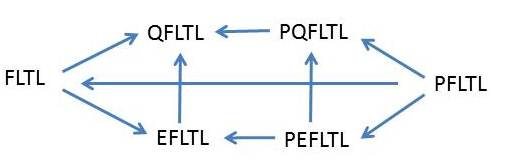
\includegraphics[height=1.1in,width=2.7in]{FIRST.jpg}
\caption{\label{fsfr} An arrow from A to B means that logic  B is more expressive than A}
\end{center}
\end{figure}


\section{RV for First-Order Past-Time LTL and its Extension}
\label{EPLTLRV}

Runtime verification of FLTL is performed on an
input that consists of {\em events} in the form of
tuples of relations. In our notation, the input
consists of a sequence ${\cal R}[1] \, {\cal R}[2]  \ldots$,
which we earlier identified with states, where each
${\cal R}[i]$ consists of some relations. A typical use
of runtime verification restricts these relations to have,
per each state just some finite tuples, and, quite commonly, have a single tuple from a single relation per each state.
A set of assignments over the same variables, which has some fixed order
(say alphabetical) also forms a relation.

\klaus{In the text above there are some imprecisions, such as
(1) ``tuples of relations'' - relations are sets of tuples, we don't have tuples of relations. 
(2) ``${\cal R}[i]$ consists of some relations'': it is a set of
relations (I think).
(3) ``to have, per each state just some finite tuples'': tuples are finite. You mean: to contain a finite set of tuples?
(4) what is the story about a set of assignments also being a relation? Needed?
}

\subsubsection{Syntax}

\klaus{Below: (\ref{EFLTL}) was not a EPFLTL form of specification.}

Consider again the EPFLTL form
of specification, described in~(\ref{EFLTL}), restricted to the past operators. We now present the definition of EPFLTL, the final main logic proposed in this paper. 
The syntax is as follows:


\[ 
\psi \mathrm{\ where\ } r_j ( x_j) := 
\varphi_j (x_j) : j \in \{ 1 , \ldots , n \}
\]
\begin{center}
$\varphi ::= \true  \; | \;
    p ( a ) \; | \;
    p ( x ) \; | \;
    ( \varphi \wedge \varphi ) \;  |   \;
   \neg \varphi \; | \;
    \ominus \varphi \; | \;
    ( \varphi  \; \since  \; \varphi ) \; | \;
    \exists x \; \varphi$
\end{center}

\klaus{Note that $\psi$ above is not defined as a syntactic category. It should really be $\varphi$. Likewise in other parts of the paper. Perhaps too big a change now? Also, there should be
a greek letter for a specification. E.g.:

\[ 
\pi ::= \varphi \mathrm{\ where\ } r_j ( x_j) := 
\varphi_j (x_j) : j \in \{ 1 , \ldots , n \}
\]
\[
\varphi ::= ...
\]
}

\iffalse
\noindent {\bf Set Semantics.}
We now refine the semantics of the logic. Under the new definition, 
$I [ \varphi , \sigma, i ]$ is a function that returns
a set of assignments such that $\gamma \in I [ \varphi , \sigma, i ]$ 
iff $( \gamma , \sigma , i ) \models \varphi$.
This redefinition will later lead to a simple implementation 
using BDDs, where each set of assignments will be represented
as a BDD, and the Boolean operators will correspond directly 
to Boolean operators on BDDs.

In order to deal with subformulas with different sets of free
variables (hence, different domains for assignments), 
we apply a projection and an extension operator to assignments
over a subset of the variables. Let $\Gamma$ be
a set of assignments over the variables $W$, and
$U \subseteq W$.
Then $\proj ( \Gamma , U )$ (for ``projecting {\em out}'' or  ``hiding''
the variables $U$)
is the largest set of assignments over 
$W \setminus U$, 
each agreeing with some
assignment of $\Gamma$ on all the variables in $W \setminus U$.
Let $U \cap W = \emptyset$, then
$\ext ( \Gamma , U )$ is the largest set of assignments
over $W \cup U$, where each such assignment agrees 
with some assignment in $\Gamma$ on the
values assigned to the variables $W$. 
This means that we extend $\Gamma$ by
adding arbitrary values to the variables in $U$ from their domains.
Then $\proj ( \ext ( \Gamma , U ) , U ) = \Gamma$ holds.
We define the union and intersection operators on sets of
assignments, even if they are defined over non identical
sets of variables. 
In this case, the assignments are extended
over the union of the variables. Thus, if $\Gamma$ is a
set of assignments over $W$ and $\Gamma'$ is
a set of assignments over $W'$, then
$\Gamma \; \bigcup \;  \Gamma'$ is defined as $\ext (\Gamma , W' \setminus W ) \cup
\ext ( \Gamma' , W \setminus W' )$ and
$\Gamma \; \bigcap \; \Gamma'$ is $\ext (\Gamma , W' \setminus W ) \cap
\ext ( \Gamma' , W \setminus W' )$.  Hence, both are defined
over the set of variables $W \cup W'$.



%We define $\mathbf{F}$ and $\mathbf{T}$ as special constants
%in order to interpret formulas without free variables.
%They are the complement of each other.
%When combined with set operators (complementation, union, intersection),
%$\mathbf{F}$ behaves as the empty set, hence is idempotent to
%union. Accordingly, $\mathbf{T}$ is idempotent to intersection.
\fi

\klaus{One may of course ask whether the following section on the 
set semantics is needed. Maybe it is needed, since we probably need a semantics. Something to consider.}

\subsubsection{Semantics}

We denote by $A_{\vars ( \varphi )}$ the set of all possible assignments
of values to the variables that appear free
in $\varphi$. Thus,
$I [ \varphi, {\cal R} , i] \subseteq A_{\vars ( \varphi )}$.
To simplify definitions, we add
a dummy position $0$ for sequence $\sigma$ (which starts with $s_1$), 
where every formula is interpreted as an empty set.
Observe that the value $\emptyset$ and $\{ \epsilon \}$, behave
as the Boolean constants $0$ and $1$, respectively.
The set semantics is defined as follows, where $i \ge 1$.

\klaus{Above: assignments are introduced without any gentle introduction. Remember: you are not communicating with Moshe Vardi. You are communicating with John Fingelstein who had three glasses of wine at dinner.}

\klaus{Above: $I [ \varphi, {\cal R} , i]$ is introduced out of the blue without any explanation.}

\begin{itemize}
\item $I [ \varphi , {\cal R} , 0 ] = \emptyset$.
\item $I [ \true , {\cal R} , i ] = \{ \epsilon \}$.
\item $I [ p ( a ) , {\cal R} , i ] =$ if $p ( a ) \in \sigma [ i ]$ then
$\{ \epsilon \}$ else $\emptyset$.
\item $I [ p ( x ) , {\cal R} , i ] = \{ [ x \mapsto a ] | p ( a ) \in
\sigma [ i ] \}$.
%\item $I [ \true , \sigma , i ] = D^n$.
%\item $I [ ( \varphi \vee \psi ) , \sigma , i ] = 
%I [ \varphi , \sigma , i ] \cup I [ \psi , \sigma , i ]$.
\item $I [ ( \varphi \wedge \psi ) , \sigma , i ] = 
I [ \varphi , {\cal R} , i ] \;  \bigcap \; I [ \psi , \sigma , i ]$.
\item $I [ \neg \varphi , {\cal R} , i ] = 
A_{\vars ( \varphi )} \; \setminus \; I [ \varphi , {\cal R} , i ]$.
\item $I [ ( \varphi \; \since \; \psi ) , {\cal R} , i ] = 
I [ \psi , {\cal R}, i ] \; \bigcup \;
( I [ \varphi , {\cal R} , i ] \bigcap 
I [ (\varphi \since \psi ) , {\cal R} , i - 1 ] )$.
\item $I [ \ominus \varphi , {\cal R} , i ] = I [ \varphi , {\cal R} , i-1 ]$.
\item $I [ \exists x \; \varphi , \sigma , i ] = 
\proj ( I [ \varphi , {\cal R} , i ] , \{ x \} )$.
\item $I [ \psi \mathrm{\ where\ } r_j ( x_j) := 
\varphi_j (x_j) : j \in \{ 1 , \ldots , n \} , {\cal R} , i ] = 
 I [ \psi , {\cal Q} ] $ where ${\cal Q} = {\cal R} \cup
\{ r_j | r_j [ i ] =  I [ 
\varphi_j , {\cal Q} , i ] \}$
\end{itemize}

\klaus{Above: as the semantics is presented, it looks as if 
the `$\psi\ where ...$' is just another subformula.}

\klaus{Above: hide is not defined.}

\klaus{Above: the semantics of $p(a)$ and $p(x)$ do not refer to 
${\cal R} $.}

In the last item, the extended model ${\cal Q}$ appears both on the left and the right of the equality sign. It is well defined because of Lemma~\ref{samesame}.

\subsubsection{Runtime Verification Algorithm for PFLTL}

We start by describing an algorithm for monitoring 
PFLTL properties, first presented in~\cite{HPU} and implemented
in the tool~\dejavu. 
Instead of storing the data values occurring in events, 
we enumerate these data values as soon as we see them and use Boolean
encodings of this enumeration, represented as BDDs.
For example, if the runtime verifier sees the input 
events 
$\mathit{open}(\text{``a''})$, 
$\mathit{open}(\text{``b''})$, 
$\mathit{open}(\text{``c''})$, 
it will encode them as
$000$, $001$ and $010$ (say, we use 3 bits $b_0$, $b_1$ and $b_2$
to represent each enumeration, with $b_2$ being the most significant bit).
%
A Boolean representation of the {\em set} of values 
$\{\text{``a''},\text{``b''}\} $ would be equivalent to a Boolean function $(\neg b_1 \wedge \neg b_2)$ that returns 1 for $000$ and $001$ (the value
of $b_0$ can be arbitrary).

%

Since we want to be able to deal with infinite domains
(where only a finite number of elements may appear in a given observed prefix) and maintain the ability to perform
complementation, unused enumerations represent the
values that have not been seen and their relations
to all other values. The algorithm maintains that these unseen values are correctly represented, as shown in~\cite{HPU}. In fact, it is sufficient to have just one enumeration representing these values per each variable of the LTL formula. However, it is important to guarantee that at least one such enumeration
exists. We guarantee that by preserving the enumeration $11\ldots11$, i.e., the highest Boolean representation,
to represent values not yet seen.
We present here only the basic algorithm. For versions that
allow extending the number of bits used for enumerations and garbage collection of enumerations, consult~\cite{HP}.

Our preferred representation of a set of values 
(assignments) is as an Ordered Binary Decision
Diagram (OBDD, although we write simply BDD)~\cite{Bryant}.
A BDD is essentially a compact representation 
of a Boolean tree, where compaction glues together isomorphic subtrees. Each non-leaf node is labeled with one of the
Boolean variables $b_0,\ldots,b_{k-1}$ (where $k$ is the number of bits used to represent the values of a variable). A non-leaf node $b_i$ 
is the source of two 
arrows leading to other nodes, representing respectively that the node has the value 0 (false) or 1 (true).
%A dotted-line arrow represents that $b_i$ has the Boolean value $0$, while a thick-line 
%arrow represents that it has the value $1$. 
The nodes in the DAG have the
same order along all paths from the root. However, some of the nodes may be
absent along some paths, when the result of the Boolean function does not 
depend on the value of the corresponding Boolean variable. Each path leads 
to a leaf node that is marked by either a $0$ or a $1$, representing the 
Boolean value returned by the function for the Boolean values on the path.

The use of BDDs can be replaced by other representations that
can compactly and efficiently represent sets of values (e.g., ZDDs), and to which one can apply set operations like complementation, intersection, union (which are simply negation, conjunction and disjunction
in BDDs) and projection (for the quantification).
The marriage of BDDs and Boolean enumeration is in particular
efficient, since collections of adjacent Boolean enumerations tend to compact well.



\iffalse %%%%%
The definition of the {\em since} operator $S$ can be rewritten in a standard
way such that it refers only to the positions $i$ and $i-1$ in
the sequence $\sigma$. 
This is based on the
fact that according to the semantics of {\em since},
$(\varphi \, \since \, \psi) = ( \psi \vee (\varphi \wedge \ominus 
(\varphi \, \since \, \psi )))$.
This will serve in the
implementation to work with only two versions of
the sets of assignments, for the current and previous state:

\begin{itemize}
\item $( \gamma , \sigma , i ) \models ( \varphi \, \since \, \psi )$ if
$( \gamma |_{\vars ( \psi )} , \sigma , i ) \models \psi$ or $i>1$,
$( \gamma |_{\vars ( \varphi )} , \sigma , i ) \models \varphi$, and 
$( \gamma , \sigma , i-1 ) \models ( \varphi \, \since \, \psi )$.
\end{itemize}
\fi %%%%%
 
%The rest of the operators are defined as follows:
%$\false = \neg \true$, $\forall x \; \varphi = \neg \exists x \neg \varphi$,
%$(\varphi \vee \psi) = \neg ( \neg \varphi \wedge \neg \psi )$.
%We can also define the following useful operators:
%$P \varphi = (\true \, \since \, \varphi)$ (for ``previously''),
%$( \varphi \, R \, \psi ) = \neg ( \neg \varphi \, \since \, \neg \psi )$ 
%(the dual of the Since operator), and
%$H \varphi = ( \false \, R \, \varphi )$ (for ``always in the past'').

%\noindent {\bf Set Semantics.}
%It helps to represent the algorithm to 
%redefine the semantics of
%the logic in terms of sets of assignments satisfying a formula.
%Then $I [ \varphi , \sigma, i ]$ is a function that returns
%a set of assignments such that $\gamma \in I [ \varphi , \sigma, i ]$ 
%%Then a BDD for a set containing the values ``de'' and ``af''
%%(2nd and 3rd values)
%will return $1$ for $01$ and $10$. If the Boolean function is over
%$b_0$ (for most significant bit) and $b_1$ (for least significant), 
%then this is the Boolean function 
%$(\neg b_0 \wedge b_1) \vee (b_0 \wedge \neg b_1)$.

Given some ground predicate $p ( a )$ observed in the execution 
matching with $p ( x )$ in the monitored property,
let $\lookup ( x, a )$ be the enumeration of $a$. If this
is $a$'s first occurrence, then it will be assigned a new enumeration.
Otherwise, $\lookup$ returns the enumeration that $a$ received before. We can use a counter, for each variable $x$, counting the number of different values appearing so far for $x$. When a new value appears, this counter is incremented, and the value is converted to
a Boolean representation. Enumerations that were not yet used represent
the values not seen yet. 
%In particular, we always leave at least
%one enumeration, $11\ldots 11$, for this purpose.
%In the next section we introduce data reclaiming, which allows 
%reusing enumerations for values that no longer affect the checked 
%property. 
%This involves a more
%complicated enumeration mechanism.


The function $\bddset (x, A)$ returns
a BDD that represents the set of assignments where $x$ is mapped to 
(the enumeration of) $v$ for
$v \in A$. This BDD is independent
of the values assigned to any variable
other than $x$, i.e., they can have any value.
For example, assume that we use the three Boolean variables (bits) $x_0$, $x_1$ and $x_2$
for representing enumerations over $x$ (with $x_0$ being the least significant bit), and
assume that $A = \{ a , b \}$, 
$\lookup ( x, a ) = 000$, and $\lookup ( x , b ) = 001$.
Then $\bddset ( x , A )$ is a BDD representation of the Boolean function 
$(\neg x_1 \wedge \neg x_2)$. 
%But the BDD function will be independent of the values of Boolean variables
%representing other variables.
%Notice that $p ( x )$ is
%equivalent, and is represented as $\exists y \, \exists z \, p ( x )$
%when the variables used in the formula are $x$, $y$ and $z$.

Intersection and union of sets of assignments are translated simply
to conjunction and disjunction of their BDD representation,
respectively, and complementation
becomes BDD negation. We will denote
the Boolean BDD operators as $\bddwedge$, $\bddvee$ and $\bddneg$.
To implement the existential (universal, respectively) operators, 
%as in the interpretation of $\exists x \; \varphi$, 
we use the BDD existential (universal, respectively) operators over
the Boolean variables that represent (the enumerations of) the values of $x$. 
%Thus, $x$ is translated into
%is represented using the Boolean variables $x_1$, $x_1, \ldots x_{k}$ into 
Thus, if $B_{\varphi}$ is the BDD representing
the assignments satisfying $\varphi$ in
the current state of the monitor, then 
$\bddexists (\langle x_0,\ldots,x_{k-1} \rangle, B_{\varphi})$
is the BDD that represents the assignments satisfying $\exists x \; \varphi$ in the current
state.
Finally, $\bfalse$ and $\btrue$  are the BDDs that return always
$0$ or $1$, respectively.

%The case where the number of bits used to represent values for
%some domains is eventually insufficient is dealt with by
%expanding the number of bits for the BDD. This will be explained later,
%but is much harder to implement, and may require a lot of overhead
%to update the BDDs while online computation is monitored. This
%may be unnecessarily, as we can assign a large number of bits
%a priory, where these bits represent a set of values that is
%exponentially larger.

The algorithm shown below works similarly to the algorithm for the 
propositional case shown in
Section~\ref{LTLruntime}. That is,
it operates on two vectors (arrays) of values indexed by subformulas: 
$\old$ for the state before that event, and
$\current$ for the current
state (after the last seen event).
However, while in the propositional case the vectors contain Boolean values, here
they contain BDDs. The temporal relations are
represented by
sets of events, each being a tuple of one of the relations. Thus, $R_k [ i ]$ refers to the set
of tuples of the relation $R_k$ at time instant $i$. Often (and in our implementation), the set of events consists of a singleton tuple of a single relation.
The algorithm follows.

\begin{enumerate}
\item Initially, for each subformula $\varphi$,
%$B ( \varphi , \current ) = \bfalse$.
$\current ( \varphi ) := \bfalse$.
\item Observe a new state (as a set of ground predicates) $s_i$ as input. 
\item Let $\old := \current$.
\item Make the following updates for each subformula. If $\varphi$ is
      a subformula of $\psi$ then $\current ( \varphi )$ is updated before 
      $\current ( \psi )$.
\begin{itemize}
  \item $\current ( \true ) := \btrue$.
  \item $\current ( p_k ( a ) )$ := if $R_k [ i ] ( a )$ then
  $\btrue$ else $\bfalse$.
  \item $\current ( p_k ( x ) )$ :=
     $\bddset ( x ,  \{ a \ | \ R_k[i] ( a  ) \} )$.
  \item $\current ( ( \varphi \wedge \psi ) ) := 
  \bddwedge ( \current ( \varphi ) , \current ( \psi ))$.
  \item $\current ( \neg \varphi  ) := \bddneg ( \current ( \varphi ))$.
  \item $\current ( ( \varphi\ \since\ \psi ) ) := \\ 
  \bddvee ( \current ( \psi  ) , \bddwedge ( \current ( \varphi ) ,
      \old ( ( \varphi \ \since \ \psi ))))$.
%DAP: I removed the \; around \since, since it penetrated the 2nd column!
  \item $\current ( \ominus \; \varphi ) := \old ( \varphi )$.
  \item $\current ( \exists x \; \varphi ) := 
  \bddexists (\langle x_0,\ldots,x_{k-1} \rangle, \current ( \varphi ))$.
\end{itemize}
\item Goto step~2.
\end{enumerate}

\subsubsection{Runtime Verification Algorithm for EPFLTL}

We extend now the algorithm to capture EPFLTL.
The auxiliary relations $r_j$ extend the model, and we need to keep 
a BDDs representing $\current ( r_j )$ and
$\old (r_j)$ for each relation $r_j$. We also need to calculate the subformulas $\varphi_i$ that appear in
a specification, as part of the runtime verification,
as per the above FPLTL algorithm. The auxiliary relations $r_j$ are calculated with respect to
a variable $x_j$, which is the one appearing
free in $\varphi_j$ (this can be generalized to any number of variables). However, $r_j$ can be used
as a subformula with other parameters in other rules or in the statement. Thus,
$r_j ( y )$ constructing a relation
that is the same as $r_j$, but over the variable $y$. This can be achieved by the BDD renaming function $\rename ( r_j (x_j ) , y)$, which is easy to implement in BDDs.


We then have to add
following updates between steps 3 and 4 of the above algorithm, when performing runtime verification of
$\psi$. 

\noindent \begin{description}
\item For each $r_j ( x_j ) = \varphi_j ( x_j )$:
\item{\ \ }  calculate $\current ( \varphi_j )$;
\item{\ \ }  $\current ( r_j )  := \current (\varphi_j)$;
\item{\ \ } $\current ( r_j ( y ) )$ := $\rename ( r_j(x_j) ,  y )$;
\item{\ \ } $\current ( r_j ( a ) )$ := if $\current ( r_j ) ( a )$
then $\btrue$ else $\bfalse$; 
\end{description}

\klaus{Above: $\current ( r_j ) ( a )$ has not been defined I think.}

\noindent
As in the propositional case, the evaluation order cannot be
simply top down or bottom up, since relations can appear
both on the left and the right of a definition
such as $r ( x ) := p ( x ) \vee \ominus r ( x )$. For that,
we need to use the mixed evaluation order, described in Section~\ref{LTLruntime}.













